\documentclass{report}

\usepackage{global}
\graphicspath{{/home/grybouilli/TIPE/schema/}}
\author{Nicolas GRY}

\title{Étude du mouvement du déchet}

\begin{document}
\maketitle
\tableofcontents
\newpage
\chapter{Phase de déplacement dans le champ magnétique}
\section{Mise en situation}
\subsection{Introduction des grandeurs et notations}

On considère un solénoïde caractérisé par:
\begin{itemize}
    \item Sa longueur $L$
    \item Son rayon $a$
    \item L'intensité du courant qui le traverse $i$
    \item Son nombre de spires $n$ 
\end{itemize}
Ce solénoïde engendre un champ magnétique:
 $$\vect{B} = B_r \vect{e_r} + B_z \vect{e_z}$$.
On notera indifféremment $||\vect{B}||$ et $B$.

On considère un déchet spatiale:
\begin{itemize}
    \item modélisé par un solide parallélépipède rectangle de volume $V=hlL$
    \item portant un moment magnétique $\vect{p}$
    \item de moment d'inertie $J_\theta$
    \item de masse m
\end{itemize} 
On notera indifféremment $||\vect{p}||$ et $p$.

On travaillera dans le repère cylindrique $(\vect{e_r},\vect{e_\theta},\vect{e_z})$ et on notera $(r,\theta,z)$ les coordonnées du déchet.

\subsection{Schématisation de la situation}

\begin{figure}[h]
    \centering
    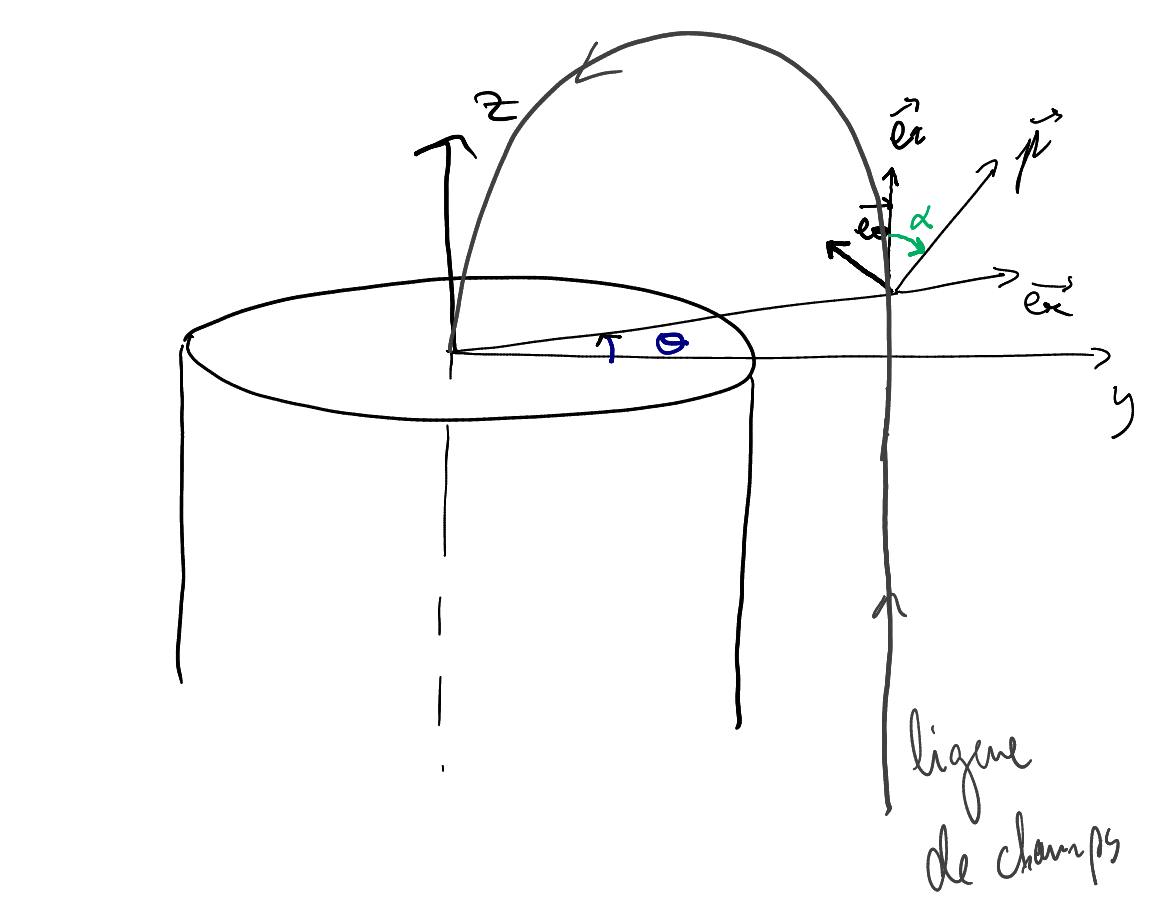
\includegraphics[scale=0.15]{schema_etude_mouvement_1.png}
    \caption{Schéma simplifié de la situation}
\end{figure}  

On imagine que le moment magnétique $\vect{p}$ forme un angle $\alpha$ avec $\vect{e_z}$. L'objectif ici est d'étudier les variations de $\alpha$ et d'évaluer le temps que met $\vect{p}$ à s'aligner avec les lignes de champs.
\newpage

\section{Introduction à la modélisation dipolaire}
\subsection{Cas du matériau paramagnétique}
Un matériau paramagnétique est un matériau qui ne possède d'aimantation naturelle; hors de tout champ magnétique, il n'a pas de moment magnétique. En effet, les moments magnétiques atomiques étant "désorganisés", le moment magnétique total du matériau est globalement nul.

Soumis à un champ magnétique, les moments magnétiques atomiques s'alignent selon le champs magnétique excitateur, provoquant un moment magnétique global. Ce phénomène confère au matériau une aimantation et on peut donc assimiler le matériau à ce moment magnétique.

\subsection{Aimantation}
L'aimantation est définie comme étant la densité volumique de moment magnétique, c'est-à-dire: $$M = \frac{\mathrm{d}m}{\mathrm{d}V}$$
où $\mathrm{d}m$ est le moment magnétique contenu dans $\mathrm{d}V$.

Dans le cas du paramagnétisme, elle représente le moment dipolaire du matériau paramagnétique considéré. On a la relation:

$$M = \chi B$$

où $B$ est l'intensité du champ magnétique extérieur auquel on soumet le matériau et $\chi$ la susceptibilité magnétique du matériau.

\section{Modélisation du matériau paramagnétique}
\subsection{Modèle de Langevin}

Dans ce modèle, Langevin fait l'hypothèse que les molécules portant le moment magnétique élémentaire sont orientées librement ce qui \textbf{limite ce modèle aux gaz}.
On considère un matériau paramagnétique comme un ensemble de N sites portant chacun un moment magnétique $\vec{m_i}$, tous indépendants mais de norme commune qu'on notera $||\vec{m_0} || = m_0$.

Dans le modèle de Langevin, on exprime alors d'abord le moment magnétique moyen du matériau $\valmoy{m}$ pour exprimer l'aimantation. La démonstration de Langevin de 1905 amène au résultat suivant pour l'aimantation moyenne du matériau qui sera colinéaire au champ magnétique auquel le matériau est soumis:

$$\valmoy{M_u} = Nm_0L(x)$$
où L est la fonction de Langevin telle que

$$L(x) = \coth(x) - \frac{1}{x} \mbox{ et on a posé } x = \frac{m_0 B}{k_B T}$$
\emph{N.B: L est donc une fonction de la température.}

Ce résultat est valable pour un champ magnétique qui s'exprime selon une direction $\vec{u}$. Dans notre cas, on a :

$$\vect{B} = B_r \vect{e_r} + B_z \vect{e_z} $$

donc : 
$$\vec{u} = \frac{B_r \vect{e_r} + B_z \vect{e_z}}{\sqrt{B_r^2 + B_z^2}}$$

Et on a une aimantation moyenne pour un matériau plongé dans le champ magnétique du solénoïdé fini:
\rule{\textwidth}{0.4pt}
    $$\vec{M} = Nm_0L(x) \frac{B_r(r,z) \vect{e_r} + B_z(r,z) \vect{e_z}}{\sqrt{B_r(r,z)^2 + B_z(r,z)^2}} $$
avec $$L(x) = \coth(x) - \frac{1}{x} \mbox{ et on a posé } x = \frac{m_0 \sqrt{B_r(r,z)^2 + B_z(r,z)^2}}{k_B T}$$
\rule{\textwidth}{0.4pt}

\emph{Références pour les calculs : }
\begin{itemize}
    \item Démo du modèle de Langevin  : \url{https://fr.wikipedia.org/wiki/Paramagn%C3%A9tisme}
    \item Infos sur la fonction de Langevin \url{https://fr.wikipedia.org/wiki/Fonction_de_Langevin}
    \item Effet de Zeeman et calcul du moment magnétique d'un électron : \url{https://fr.wikipedia.org/wiki/Effet_Zeeman}
\end{itemize} 

\subsection{Modèle paramagnétique de Pauli pour les métaux}
Dans ce modèle, la susceptibilité du matériau est déterminée à partir du comportement des électrons de conduction et on utilise la répartition statistique de Fermi-Dirac sur les fermions, appliquée aux électrons des atomes des métaux. 

On modélise un morceau de matériau métallique par un "gaz d'électrons". L’idée de base est considérer que les électrons sont totalement délocalisés et l’influence des noyaux et des autres électrons est moyenné de telle sorte que le potentiel vu par par un électron est constant. 

On prend pour système un parallélépipède rectangle de volume $V = l*L*h$.
L'équation de Schrödinger devient:
$$\Delta \Psi = 0$$

Pour l'étude des solides, on utilise des conditions périodiques dites de Born-von Karman, et on arrive à montrer qu'il y a discrétisation des vecteurs d'onde qui vérifient la relation:
$$E = \frac{\hbar ||\vect{k}||^2}{2m_e}$$
où $m_e$ est la masse d'un électron.

\rule{\textwidth}{0.4pt}

\begin{center}
\textbf{Définition: Énergie de Fermi}
    
    C’est l’énergie maximale atteignable par un fermion dans l’état fondamental du système de N fermions.

\emph{N.B.: Un fermion est une particule de spin demi-entier, par exemple un électron.}    
\end{center}

\rule{\textwidth}{0.4pt}

À l'énergie de Fermi $E_F$ on associe le vecteur d'onde de Fermi $\vect{k_F}$. Les niveaux d'énergie d'un atome se remplissant par ordre croissant, par définition, $\vect{k_F}$ correspond au niveau d'énergie maximal. Chaque état du système à $N_e$ électrons possède deux électrons de spins opposés et sont associés à des vecteurs d'ondes variant entre $-\vect{k_F}$ et $\vect{k_F}$. On peut donc avec les conditions de Born-von Karman montrer que :

$$\frac{N_e}{V} = \frac{k_F^3}{3\pi^2}$$

Ce qui permet d'exprimer l'énergie de Fermi pour n'importe quel gaz d'électrons:


    $$E_F(N_e) = \frac{\hbar}{2m_e} \left(\frac{3\pi^2N_e}{V}\right)^{2/3}$$
avec donc:
    \begin{itemize}
        \item $\hbar$ la constante de Planck
        \item $m_e$ la masse d'un électron
        \item $N_e$ le nombre d'électrons dans le gaz d'électron qui modélise le métal
        \item $V$ le volume de matériau considéré
    \end{itemize}
(\emph{source: }\url{https://crppwww.epfl.ch/physgen4/repository/Notes_04.05.2009.pdf})

\rule{\textwidth}{0.4pt}
\begin{center}
Le paramagnétisme de Pauli donne alors le résultat suivant pour l'\textbf{aimantation totale du matériau}:

$$M = \frac{3\mu^2 N_e B}{2 E_F(N_e)}$$

\begin{itemize}
    \item $\mu_B$ le magnéton de Bohr
    \item $N_e$ le nombre de sites magnétiques par unité de volume
    \item $B$ la norme du champ magnétique extérieur
    \item $E_F(N_e)$ Énergie de Fermi pour un gaz de $N_e$ électrons
\end{itemize}    
\end{center}

\rule{\textwidth}{0.4pt}
\subsection{Détermination de moments magnétiques pour divers métaux}
\subsubsection{Approche générale}
\url{https://www.google.com/url?sa=t&rct=j&q=&esrc=s&source=web&cd=&ved=2ahUKEwi8qsLcgsHwAhVk8-AKHWimDEsQFjAHegQICBAD&url=https%3A%2F%2Felearn.univ-oran1.dz%2Fpluginfile.php%2F55565%2Fcourse%2Foverviewfiles%2FParamagnetisme%2520de%2520Pauli.pdf%3Fforcedownload%3D1&usg=AOvVaw0VCRp_iYkn5Ij4NKFHUNlp}

Dans le doc suivant, on a un tableau avec les densité de populations d'électrons pour plusieurs éléments ce qui permet de trouver le fameux $N_e$ pour un volume défini.

(\url{https://www.google.com/url?sa=t&rct=j&q=&esrc=s&source=web&cd=&cad=rja&uact=8&ved=2ahUKEwiy1IPUosHwAhWIB2MBHUGiAtAQFjACegQIBRAD&url=http%3A%2F%2Firamis.cea.fr%2FPhocea%2Ffile.php%3Fclass%3Dcours%26file%3D%2Fcyrille.barreteau%2FPhysique_du_Solide_Barreteau_Chapitre3.pdf&usg=AOvVaw1BqPW51Q1njSGLnC4VscLL})

Maintenant, comme on est des bons gars, on va montrer quand même comment ces valeurs ont été trouvées et par chance, juste avant le tableau, y a un raisonnement rapidement détaillé lol.

D'abord, dans le modèle du gaz de fermions, notamment du gaz d'électrons, ce sont les électrons de valence qui participent à constituer le moment magnétique globale observé pour un ensemble d'atomes, les électrons de coeur étant considérés comme inertes.

On étudie la population des atomes d'une maille d'un réseau cristallin constituant le matériau considéré, on multiplie cette population par le nombre d'électrons de valence pour l'atome considéré et on obtient le nombre d'électrons actifs dans la maille. Il reste à déterminer le volume de la maille en question pour avoir la densité d'électrons pour le matériau choisi. (vive la cristallo \smiley{})
\subsubsection{Pour un matériau en aluminium}

La maille d'aluminium a une configuration cubique à face centrée de rayon atomique $r=1,43\,\AA$ donc $$4r=\sqrt{2}a \iff a = 2\sqrt{2}r \mbox{, ie :} \, a = 4,04\,\AA$$
et la maille a un volume de $v = 66,2 \,\AA^3$. L'aluminium a trois électrons de valence et la maille d'aluminium a une population de 4 donc finalement:
$$n_{Al} = 0,181 \text{ électrons} / \AA^3$$

\subsubsection{Pour un matériau en zinc}
Le zinc est organisé en une maille hexagonal compacte de rayon atomique $r=1,35 \,\AA$ et $a = b = 2r \mbox{ et }c = 4r.\sqrt{(2 / 3)}$ donc:
$$a=b=2,70\,\AA$$
$$c=4,41\,\AA$$
et la maille a un volume de $v = 167\,\AA^3$. Le zinc a 12 électrons de valence et la maille de zinc a pour population 2 donc finalement:
$$n_{Zn} = 0,143 \text{ électrons} / \AA^3$$
\subsubsection{Pour un matériau en titane}
Le titane est organisé en une maille hexagonal compacte de rayon atomique $r=1,4 \,\AA$ et $a = b = 2r \mbox{ et }c = 4r.\sqrt{(2 / 3)}$ donc:
$$a=b=2,80\,\AA$$
$$c=4,57\,\AA$$
et la maille a un volume de $v = 186\,\AA^3$. Le titane a 4 électrons de valence et la maille de titane a pour population 2 donc finalement:
$$n_{Ti} = 0,043 \text{ électrons} / \AA^3$$

\section{Étude littérale du mouvement}
\subsection{Étude de l'alignement angulaire du déchet}

\ulbf{Système}: {débris assimilé à un moment magnétique solide $\vect{p}$ de moment d'inertie $J_\theta$}

\ulbf{Référentiel}: En lien avec le solénoïde, supposé galiléen (raisonnable au regard de la durée de l'expérience)

\ulbf{Conditions initiales}

À t = 0, on suppose que le déchet est incliné d'un angle $\alpha_0$ par rapport à l'axe de révolution du solénoïde. On suppose également la vitesse angulaire $\phder{\alpha}$ du déchet nulle à t = 0, ce qui est raisonnable puisque le déchet est dénué de tout mouvement dû au champ $\vect{B}(r,z)$ lorsqu'il n'y est pas soumis, i.e. à t = 0.

\ulbf{Bilan des forces}

\emph{NB : Il ne faut pas oublier durant cette étude que $\vect{B}$ dépend de r et de z, les variables du répère cylindrique défini dans le cadre de l'étude.}

Force magnétique :
$$\vec{F_B} = \vect{\text{grad}}(\vect{p}.\vect{B})$$

\ulbf{Théorème du moment cinétique}

Projeté selon $\vect{e_\theta}$ :
\begin{align*}
J_\theta \derived{\alpha}{t} &= \vect{\MM}(\vect{F_B}) . \vect{e_\theta} \\
&= (\vect{p} \wedge \vect{B}).\vect{e_\theta}\\
&= pB_r \cos(\alpha) - pB_z\sin(\alpha)
\end{align*}

On obtient l'équation différentielle suivante:

\rule{\textwidth}{0.4pt}
\begin{center}
\ulbf{Équation différentielle du 2$^{nd}$ ordre non-linéaire à second membre non-constant:}
$$\derived{\alpha}{t} + \frac{pB_z}{J_\theta}\sin(\alpha) = \frac{pB_r}{J_\theta} \cos(\alpha)$$    
\end{center}

\rule{\textwidth}{0.4pt}

\subsubsection{Étude de la fin de l'alignement angulaire}
On se place en premier dans la situation où $\alpha$ est considéré petit. On a alors:
$$\derived{\alpha}{t} + \frac{pB_z}{J_\theta}\alpha = \frac{pB_r}{J_\theta} $$

On pose $$\omega_0 = \sqrt{\frac{pB_z}{J_\theta}}$$

\ulbf{Solution générale de l'équation homogène associée}

$$\alpha_h(t) = A \cos(\omega_0 t + \varphi)$$

$\, \text{ avec } A \text{ et } \varphi \text{ des constantes d'intégrations}$.

\ulbf{Solution particulière de l'équation}

$$\alpha_p(t) = \frac{B_r}{B_z}$$


\ulbf{Solution générale de l'équation}

$$\alpha(t) = A \cos(\omega_0 t + \varphi) + \frac{B_r}{B_z}$$

\ulbf{Détermination des constantes d'intégration avec les conditions initiales}

Avec:
$$\alpha(0) = \alpha_0$$
$$\derive{\alpha}{t} (0) = 0$$

On en déduit : 
$$A = \alpha_0  - \frac{B_r}{B_z}$$
$$\varphi \equiv 0 \left[\pi\right] $$ 

Et donc finalement :\newpage

\rule{\textwidth}{0.4pt}
\begin{center}
\ulbf{Équation de l'angle formé entre $\vect{p}$ et $\vect{e_z}$}
    $$\alpha(t) = \left(\alpha_0  - \frac{B_r(r,z)}{B_z(r,z)}\right) \cos(\omega_0 t) + \frac{B_r(r,z)}{B_z(r,z)}$$    

\begin{itemize}
    \item pulsation d'oscillation du système : $\omega_0 = \sqrt{\frac{pB_z}{J_\theta}}$
    \item moment d'inertie du solide : $J_\theta = \frac{m(h^2+l^2+L^2)}{12}$
\end{itemize}
\end{center}

\rule{\textwidth}{0.4pt}

\subsubsection{Étude de l'alignement angulaire : Résolution numérique de l'équation différentielle}

\subsection{Étude du déplacement du moment dans le champ magnétique}

On passe ici à l'étude du déplacement du débris le long d'une ligne de champs. Pour cela, on modélise le débris comme un volume étant délimité par une surface fermée $S$ et doté d'une masse m.

\ulbf{Système}: {Débris assimilé à moment magnétique $\vect{p}$}

\ulbf{Référentiel}: En lien avec le solénoïde, supposé galiléen (raisonnable au regard de la durée de l'expérience)

\ulbf{Conditions initiales}

À t = 0, on suppose que le déchet est animé d'une vitesse initiale $\vect{v_0}$.

\ulbf{Hypothèse}

On travaille d'abord sans considérer la force d'attraction gravitationnelle entre le solénoïde et le débris.

\ulbf{Bilan des forces}

\emph{NB : Il ne faut pas oublier durant cette étude que $\vect{B}$ dépend de r et de z, les variables du répère cylindrique défini dans le cadre de l'étude.}

\underline{Force magnétique d'aimantation :} 
$$\vect{F} = \vect{grad}(\vect{p}.\vect{B})$$

On commence les calculs en supposant $\vect{p}$ constant.

\ulbf{Principe fondamental de la dynamique}

On considère qu'il n'y a pas de perte de masse ce qui permet d'écrire le PDF sous sa forme bien connue:

$$m\derived{\vect{OG}}{t} = \vect{F}$$


\section{Problèmes possibles}
Comme le matériau à l'origine n'a pas de moment magnétique, quand on va enter en contact avec le champ du solénoïde, il va suivre les lignes de champs et se retrouver dans le solénoïde. Problème? Il risque de ressortir expulsé avec une puissance vraiment énorme.
\end{document}